\chapter{Waves}
Wave \bf{speed} \(v\) is the distance the wave profile travels per unit time, given by
\begin{equation*}
	v = f\lambda = \f{\lambda}{T}
\end{equation*}
\begin{itemize}
	\item \(f\) is the \bf{frequency}, the number of oscillations per unit time
	\item \(\lambda\) is the \bf{wavelength}, the distance between two adjacent points oscillating in phase
	\item \(T\) is the \bf{period}, the time taken for a point on the wave to complete one oscillation
\end{itemize}

\section{Progressive waves}
\begin{definition}{Progressive wave}{wave}
	A disturbance that propagates, carrying energy without physically transferring wave particles.
\end{definition}

\subsection{Wave graphs}
\begin{figure}[htpb]
	\centering
	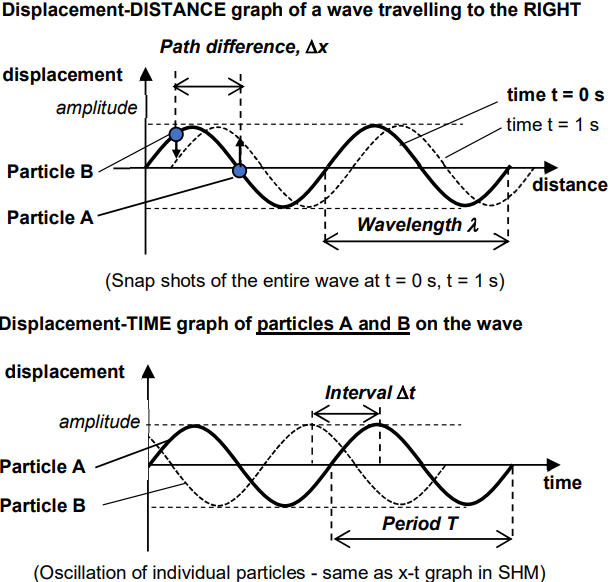
\includegraphics[width=\textwidth]{assets/wave-graphs.png}
	\caption{Wave graphs}
	\label{fig:wave-graphs}
\end{figure}

\bf{Displacement-distance graphs} take a `snapshot' of the wave at a particular instant \(\implies\) get \(\lambda\).
\it{Translate} the graph to get the wave profile at a later instant and find each point's direction of travel.
\[\Delta\phi = 2\pi\f{\Delta x}{\lambda}\]

\bf{Displacement-time graphs} show how one point on the wave oscillates with time \(\implies\) get \(T\).
The gradient \(\odv{y}{t}\) gives the speed of the point: \num{0} at the amplitude, extreme at the eq.~pos.
\[\Delta\phi = 2\pi\f{\Delta t}{T}\]

\subsection{Wave energy and intensity}
\begin{definition}{Intensity}{intensity}
	Rate at which energy is transported by the wave \it{per unit area} across
	a surface normal to direction of energy transfer. [\unit{\watt\per\square\meter}]
	\[\text{intensity} = \f{\text{power}}{\text{area}}\]
\end{definition}
Because \(E = \f{1}{2}m\omega^2{x_0}^2\),
\begin{align*}
	\text{energy}    & \propto \text{amplitude}^2 \\
	\text{intensity} & \propto \text{amplitude}^2
\end{align*}
For a wave from a \bf{point source},
\begin{align*}
	\text{intensity} & = \f{\text{power}}{\text{area}} = \f{P}{4\pi r^2} \\
	                 & \propto \lf{1}{r^2}
\end{align*}



\subsection{Transverse waves}
\begin{definition}{Transverse wave}{transverse}
	A \bf{transverse wave} is one in which points of disturbance oscillate about their eq.~pos.~\it{perpendicular}
	to the direction of energy propagation.
\end{definition}

\bf{EM waves} are transverse waves made up of mutually perpendicular \(\va{E}\) and \(\va{B}\) fields
perpendicular to the direction of energy propagation.
\begin{itemize}
	\item EM waves do not need a propagation medium; they \it{can propagate through vacuums}.
	\item EM waves travel at \(c = \qty{3.00e8}{\meter\per\second}\) in a vacuum.
\end{itemize}
\begin{table}[htpb]
	\centering
	\begin{tabular}{l l}
		\toprule
		type               & approximate \(\lambda\)              \\
		\midrule
		\bf{g}amma         & \(\qty{1e-15}{\meter}\)              \\
		\bf{x}-ray         & \(\qty{1e-10}{\meter}\)              \\
		\bf{u}ltraviolet   & \(\qty{1e-8}{\meter}\)               \\
		\bf{v}isible light & \(\qtyrange{400}{700}{\nano\meter}\) \\
		\bf{i}nfrared      & \(\qtyrange{0.7}{1}{\milli\meter}\)  \\
		\bf{m}icrowave     & \(\qty{1e-2}{\meter}\)               \\
		\bf{r}adio         & \(\qty{1e0}{\meter}\)                \\
		\bottomrule
	\end{tabular}
	\caption{EM spectrum}
	\label{tab:em-waves}
\end{table}

\begin{definition}{Polarisation}{polarisation}
	The phenomenon where vibrations in a transverse wave are \it{restricted to one direction},
	normal to the direction of energy transfer.
\end{definition}
\begin{marginfigure}
	\centering
	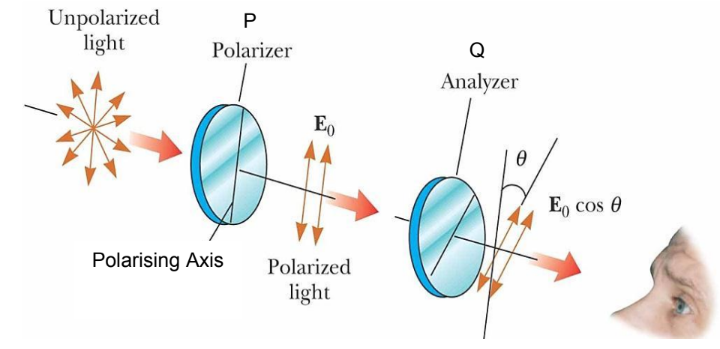
\includegraphics[width=\textwidth]{assets/polarise.png}
	\caption{Polarisation of light}
	\label{fig:polarise}
\end{marginfigure}
For a wave passing through two polarisers with an angle \(\theta\) between them\sidenote{The first polariser only allows vibrations parallel to its normal},
\[I_\text{result} = I_0 \cos^2\theta\]

\subsection{Longitudinal waves}
\begin{definition}{Longitudinal wave}{longitudinal}
	A \bf{longitudinal wave} is one in which points of disturbance oscillate about their eq.~pos.~\it{parallel}
	to the direction of energy propagation.
\end{definition}
At points where \(\text{displacement} = y = 0\),
\begin{itemize}
	\item \bf{compressions}	are regions where particles are closest together; particles before it have \(+y\) and particles after have \(-y\).
	\item \bf{rarefactions}	are regions where particles are furthest apart; particles before it have \(-y\) and particles after have \(+y\).
\end{itemize}
